% scenarios2.tex
% --
% Benjamin Williams <eeu222@bangor.ac.uk>
% Mud Dog Creative (Software Hut, Group #1)



% We want this to be an article
\documentclass[pdftex,a4paper,10pt,titlepage]{article}

% Outline the packages to be used (natbib, fancyhdr, url, geometry, hyperref)
\usepackage[utf8]{inputenc}
\usepackage[round,authoryear,sort]{natbib}
\usepackage{fancyhdr}
\usepackage{geometry}
\usepackage[hidelinks]{hyperref}
\usepackage[anythingbreaks]{breakurl}
\usepackage{titlesec}
\usepackage{graphicx}
\makeatletter
\usepackage{color}
\definecolor{lightgray}{rgb}{0.95, 0.95, 0.95}
\definecolor{darkgray}{rgb}{0.4, 0.4, 0.4}
%\definecolor{purple}{rgb}{0.65, 0.12, 0.82}
\definecolor{editorGray}{rgb}{0.95, 0.95, 0.95}
\definecolor{editorOcher}{rgb}{1, 0.5, 0} % #FF7F00 -> rgb(239, 169, 0)
\definecolor{editorGreen}{rgb}{0, 0.5, 0} % #007C00 -> rgb(0, 124, 0)
\definecolor{orange}{rgb}{1,0.45,0.13}      
\definecolor{olive}{rgb}{0.17,0.59,0.20}
\definecolor{brown}{rgb}{0.69,0.31,0.31}
\definecolor{purple}{rgb}{0.38,0.18,0.81}
\definecolor{lightblue}{rgb}{0.1,0.57,0.7}
\definecolor{lightred}{rgb}{1,0.4,0.5}
\usepackage{upquote}
\usepackage{listings}
\lstset{breaklines=true}
% CSS
\lstdefinelanguage{CSS}{
  keywords={color,background-image:,margin,padding,font,weight,display,position,top,left,right,bottom,list,style,border,size,white,space,min,width, transition:, transform:, transition-property, transition-duration, transition-timing-function}, 
  sensitive=true,
  morecomment=[l]{//},
  morecomment=[s]{/*}{*/},
  morestring=[b]',
  morestring=[b]",
  alsoletter={:},
  alsodigit={-}
}

% JavaScript
\lstdefinelanguage{JavaScript}{
  morekeywords={typeof, new, true, false, catch, function, return, null, catch, switch, var, if, in, while, do, else, case, break},
  morecomment=[s]{/*}{*/},
  morecomment=[l]//,
  morestring=[b]",
  morestring=[b]'
}

\lstdefinelanguage{HTML5}{
  language=html,
  sensitive=true,   
  alsoletter={<>=-},    
  morecomment=[s]{<!-}{-->},
  tag=[s],
  otherkeywords={
  % General
  >,
  % Standard tags
    <!DOCTYPE,
  </html, <html, <head, <title, </title, <style, </style, <link, </head, <meta, />,
    % body
    </body, <body,
    % Divs
    </div, <div, </div>, 
    % Paragraphs
    </p, <p, </p>,
    % scripts
    </script, <script,
  % More tags...
  <canvas, /canvas>, <svg, <rect, <animateTransform, </rect>, </svg>, <video, <source, <iframe, </iframe>, </video>, <image, </image>, <header, </header, <article, </article
  },
  ndkeywords={
  % General
  =,
  % HTML attributes
  charset=, src=, id=, width=, height=, style=, type=, rel=, href=,
  % SVG attributes
  fill=, attributeName=, begin=, dur=, from=, to=, poster=, controls=, x=, y=, repeatCount=, xlink:href=,
  % properties
  margin:, padding:, background-image:, border:, top:, left:, position:, width:, height:, margin-top:, margin-bottom:, font-size:, line-height:,
    % CSS3 properties
  transform:, -moz-transform:, -webkit-transform:,
  animation:, -webkit-animation:,
  transition:,  transition-duration:, transition-property:, transition-timing-function:,
  }
}

\lstdefinestyle{htmlcssjs} {%
  % General design
%  backgroundcolor=\color{editorGray},
  basicstyle={\footnotesize\ttfamily},   
  frame=b,
  % line-numbers
  xleftmargin={0.75cm},
  numbers=left,
  stepnumber=1,
  firstnumber=1,
  numberfirstline=true, 
  % Code design
  identifierstyle=\color{black},
  keywordstyle=\color{blue}\bfseries,
  ndkeywordstyle=\color{editorGreen}\bfseries,
  stringstyle=\color{editorOcher}\ttfamily,
  commentstyle=\color{brown}\ttfamily,
  % Code
  language=HTML5,
  alsolanguage=JavaScript,
  alsodigit={.:;},  
  tabsize=2,
  showtabs=false,
  showspaces=false,
  showstringspaces=false,
  extendedchars=true,
  breaklines=true,
  % German umlauts
  literate=%
  {Ö}{{\"O}}1
  {Ä}{{\"A}}1
  {Ü}{{\"U}}1
  {ß}{{\ss}}1
  {ü}{{\"u}}1
  {ä}{{\"a}}1
  {ö}{{\"o}}1
}
%
\lstdefinestyle{py} {%
language=python,
literate=%
*{0}{{{\color{lightred}0}}}1
{1}{{{\color{lightred}1}}}1
{2}{{{\color{lightred}2}}}1
{3}{{{\color{lightred}3}}}1
{4}{{{\color{lightred}4}}}1
{5}{{{\color{lightred}5}}}1
{6}{{{\color{lightred}6}}}1
{7}{{{\color{lightred}7}}}1
{8}{{{\color{lightred}8}}}1
{9}{{{\color{lightred}9}}}1,
basicstyle=\footnotesize\ttfamily, % Standardschrift
numbers=left,               % Ort der Zeilennummern
%numberstyle=\tiny,          % Stil der Zeilennummern
%stepnumber=2,               % Abstand zwischen den Zeilennummern
numbersep=5pt,              % Abstand der Nummern zum Text
tabsize=4,                  % Groesse von Tabs
extendedchars=true,         %
breaklines=true,            % Zeilen werden Umgebrochen
keywordstyle=\color{blue}\bfseries,
frame=b,
commentstyle=\color{brown}\itshape,
stringstyle=\color{editorOcher}\ttfamily, % Farbe der String
showspaces=false,           % Leerzeichen anzeigen ?
showtabs=false,             % Tabs anzeigen ?
xleftmargin=17pt,
framexleftmargin=17pt,
framexrightmargin=5pt,
framexbottommargin=4pt,
%backgroundcolor=\color{lightgray},
showstringspaces=false,      % Leerzeichen in Strings anzeigen ?
}%
%
\makeatother



\setcounter{secnumdepth}{4}

\titleformat{\paragraph}
{\normalfont\normalsize\bfseries}{\theparagraph}{1em}{}
\titlespacing*{\paragraph}
{0pt}{3.25ex plus 1ex minus .2ex}{1.5ex plus .2ex}

% Begin the document
\begin{document}



% Define title and make it (this will include the date by default
\title{\textbf{ICP-2027 / Data Structures and Algorithms} \\ Assessment 1 – Modelling Checkout Lines}
\author{
James Jackson \\ \texttt{<eeu203@bangor.ac.uk>}
}
\maketitle



% Begin the abstract, defining what this article is about.
%\begin{abstract}
%abstract
%\end{abstract}

% Render stuff which isn't top matter on a separate page
\pagebreak




% Set up page style for fancy headers, along with the header information (and page width!)
\newgeometry{margin=1.5in}
\pagestyle{fancy}
\fancyhf{}
\lhead{Mud Dog Creative \texttt{(Group \#1)}}
\rhead{ICP-2302}
\cfoot{\thepage}

\tableofcontents
















\pagebreak
% Brief
\section {Brief}

% Quote original scenario
\begin{quote}
\textit{``Write a program that models checkout lines at a supermarket; you have to use one of the data 
structures being covered in the lectures and explain why your choice of the data structure is well 
justified. Several lines of customers should be displayed. You can add a new customer by pressing a 
key. You’ll need to determine how the customer will decide which line to join. The checkers will 
take random amounts of time to process each customer (presumably depending on how many 
groceries the customer has.) Once checked out, the customer is removed from the line. For 
simplicity, you may simulate the passing of time by pressing a key. Perhaps every key-press 
indicates the passage of one minute. (Java may have more sophisticated ways to handle time.)''
}
\end{quote}

\noindent{\rule{\textwidth}{0.4pt}}

\section{Data Structure Options}

In order to successfully model the above scenario it is essential to be able to economically perform the following functions on the data structure.
\begin{itemize}
\item Remove from front
\item Add to the end
\end{itemize}


\subsection{Array}

An array is a simple linear collection of indexable elements. 

\subsubsection{Front Removal}
In a standard array, removing the first element has a time complexity of O(n) as the remaining elements must be shifted to maintain the array’s structure to ensure that insertion and counting is easier.

\subsubsection{Insertion At Endl}
Adding an element to the end of an array is as simple as knowing the final element in the array, it has a time complexity of O(1) as there is no shifting or searching required. This is on the previso that a basic structure of no fragmentation is maintained.

\subsection{Single Linked List}

A single linked list (SLL) is a group of connected elements, each pointing to the next, the begining of the linked list points to the first element, or node, in the list.

\subsubsection{Front Removal}
All operations on an SLL start from the front so removal of the front object is O(1). All that is needed is for the front of the list to point to the second object and the first object is left for garbage collection.

\subsubsection{Insertion At Endl}
In order to reach the end of the linked list it is necessary to iterate over the entire list making this functionality  O(n), also deletion on an SLL is O(n) as after an element is deleted it’s predecessor needs updating a process which requires a further n iterations to reach the element.

\subsection{Double Linked List}

A double linked lists (DLL) is similar to that of it’s sigularly linked cousin it differs however by each node having a link to it’s previous node. So for example node 3 will naturally link to node 4 but also link to node 2.

\subsubsection{Front Removal}
As with SLL the removal of the front element is  O(1) as 1 operation is needed to reach the front and delete it.

\subsubsection{Insertion At Endl}
Unlike the SLL a DLL’s front points to both the first and last element, meaning access to the final element is O(1) it’s deletion is also O(1). Updating the predecessor is also a 1 step process as the final element links to both the beginning and it’s predecessor.

\subsection{Stack}

A stack is a data structure in which addition and removal take place at the end of the structure. It offers a first in first out method of addition and access. The FIFO model will not lend itself particularly well as it is necessary to remove the first element and add to the end.

\subsection{Queue}

A queue offers the perfect structure for this scenario as it offers the exact required functionality. A queue is an abstract data structures that offers addition to the end and removal from the beginning. A queue is fundamentally first in last out which exactly models a real world supermarket queue.

\subsubsection{Queue Implementations}

\paragraph{Cyclical Array}

Adding and removing from a queue implemented using a cyclical array offer a time complexity of O(1) but the data structure is limited (in some languages) by the original length and cannot easily grow without implementing a more time intensive methodology. Where an array falls down is in clearing the queue. I order to clear the queue it is necessary to iterate over all of the data offering a time complexity of O(m) (where m is the maximum length of the queue).

\paragraph{Linked List Variant}

Adding an element to the end of a Linked list has a time complexity of O(n) as we have to iterate over the complete list to reach the end. We can introduce a slight variation to a linked list by holding a pointer to the end node from the beginning of the list, making addition to the end O(1).
Adding, removing and clearing the linked list queue implementation are O(n), one issue is with counting the size of the queue as this can mean iterating over the queue (O(n)). We can introduce a variable to the data structure to increment length on each addition and decrement on each removal. 

\section{Design}

\subsection{Classes}
The model will be written in Javascript. Javascript does not have a library implementation of a queue or a linked list so it will be necessary to create this in order to accurately model the situation.
As well as a queue class, a supermarket class will be created to allow a programmer to suggest the number of queues required and interact with the supermarket.
\subsection{Output}
Output will be modeled using basic HTML5 elements and javascript. Each queue will have representative customers and a depiction of the number of items in the queue.
\subsection{Scenario Considerations}
In the real world when approaching a checkout a customer will take a rough guess of the number of items at the checkout and opt for the one with the fewest. It is also possible that a person is influenced by the number of customers. A customer may choose a checkout serving 1 customer with 110 items over a checkout serving 10 customers with 10 items as there are 10 separate payment times to take into account. In order to accurately model there will be a running item total for each queue as well as a constant, payment, time added to each customer. New customers will find the queue with the shortest possible time including payment time.
Customers will be added and processed in 2 seperate ways chosen by the user.
\begin{enumerate}
\item Timed - customers will be added at random intervals and their items processed at smaller fixed intervals
\item Keypress - Hitting return on the kyboard adds a customer, p or backspace processes an item.
\end{enumerate}
\pagebreak
\section{Implementation}

\subsection{Queue}

\begin{lstlisting}[language=JavaScript]
/**
  Queue stucture,
  A simple impementation of a list with 2 basic functions
  
  add
  ===
  Adds an object to the end of the list
  
  remove
  ===
  Removes the first object from the queue

*/
function Queue(){
  this.first = null;
  this.last = null;
  this  .length = 0;
  // adds a new node to the end of the queue
  this.add = function(obj){
    var newNode = {
      obj: obj,
      next: null
    }
    if(this.first === null){
      this.first = newNode;
    } else {
      this.last.next = newNode;
    }
    this.last = newNode;
    this.length++;
  }
  // removes the first node from the queue
  this.removeFromQueue = function(){
    if(this.first !== null){
      if(this.first.next === null){
        this.first = null;
        this.last = null;
      } else {
        this.first = this.first.next;
      }
      this.length--;
    }
  }
  // returns the size of the queue
  this.getSize = function(){
    return this.length;
  }
  // returns the first object in the queueu
  this.getNextInQueue = function(){
    return this.first.obj;
  }
  // returns if the queue is empty or not
  this.isEmpty = function(){
    return this.first === null;
  }

  // reduces the integer value of the first element in the queue and
  // removes it if it hits zero
  this.reduceFirst = function(){
    if(this.first !== null){
      if(this.first.obj - 1 === 0){
        this.removeFromQueue();
        return false;
      } else {
        this.first.obj--;
      }
      return true;
    }
    return false;
  }
}
\end{lstlisting}

\pagebreak

\subsection{Supermarket}


\begin{lstlisting}[language=JavaScript]
/**
  SuperMarket stucture,
  A simple impementation of a supermarket made up of a specified number of queues

*/
function SuperMarket(num_queues, payment_time){

  this.queues = new Array();
  this.shortest = 0;
  // array of integers to hold the queue lengths
  this.queueLengths = new Array();

  // initialise the queues and queue lengths
  this.init = function(){
    for(var i = 0; i < num_queues; i++){
      this.queues.push(new Queue());
      this.queueLengths.push(0);
    }
  }
  
  // find the shortest queue and assign it's index to the shortest variable
  this.findShortest = function(){
    for(var i = 0; i < num_queues; i++)
      this.shortest = (this.queueLengths[this.shortest] > this.queueLengths[i]) ? i : this.shortest;
  }
  
  // add a customer to the shortest queue
  this.addACustomer = function(){
    var newCustomer = Math.floor(Math.random() * 100) + payment_time;
    this.queues[this.shortest].add(newCustomer);
    this.queueLengths[this.shortest] += newCustomer;
    this.findShortest();

  }
  
  // remove one item from the first customer in the queue providing the queue is not empty
  this.processItems = function(){
    for(var queueCounter = 0; queueCounter < num_queues; queueCounter++){
      // if the queue is not empty
      if(!this.queues[queueCounter].isEmpty()){
        this.queues[queueCounter].reduceFirst()
        this.queueLengths[queueCounter]--;
      }
    }

  }

  // returns the queues array
  this.getQueues = function(){
    return this.queues;
  }

  // returns a string representation of the supermarket
  this.toString = function(){
    var string = "";
    for(var i = 0; i < num_queues; i++){
      string += "Queue: " + this.queues[i].getSize() + " [" + this.queueLengths[i] + "] ";
      string += "\nServing: " + this.itemsToProcess[i] + "\n";
    }
    return string;
  }
  
}
\end{lstlisting}
\pagebreak
\subsection{Model Implementation}
\subsubsection{script.js}
\begin{lstlisting}[language=JavaScript]
// create supermarket instance
var supermarket = new SuperMarket(7, 10);

//global variables for the canvas, context and image
var canvas, ctx, img;
// globals for the interval timers
var itemProcessor, customerAdder;
// keys are disabled by default
var keys = false;
// initialise the supermarket
supermarket.init();

// function to clear the canvas
function clearCanvas(){
	ctx.clearRect(0, 0, canvas.width, canvas.height);
}

// draws the queues on the canvase
function drawQueues(){
	var queues = supermarket.getQueues();
	clearCanvas();
	var i;
	// loop through each queue
	queues.forEach(function(elem, ind, array){
		for(i = 0; i < elem.getSize(); i++){
			ctx.drawImage(img, 100 * ind + 20 , 31 * i, 26, 31 );
		}
		// red text color for the shortest queue
		ctx.fillStyle = (supermarket.shortest === ind)? 'red' : 'black';
		// write the ammount of items and queue length against each queue
		ctx.fillText(supermarket.queueLengths[ind] + "[" + elem.getSize() + "]", 100 * ind, 10);
	});
}

//autoupdate function, adds customers (500ms) and processes items (100ms)
function autoUpdate(){
	keys = false;
	//process an item in each queue every 100ms
	itemProcessor = setInterval(function(){
		supermarket.processItems();
		drawQueues();
	}, 100);
	// add a customer to the shortest queue every 500ms
	customerAdder = setInterval(function(){
		if(Math.round(Math.random() * 5)){
			supermarket.addACustomer();
			drawQueues();
		}
	}, 500);
}

// function to detect the status of the radio buttons
function handleRadioClick(rad){
	// if auto is selected
	if(rad.value == "auto"){
		autoUpdate();
	} else {
		// enable keys
		keys = true;
		// stop both timers
		clearInterval(itemProcessor);
		clearInterval(customerAdder);
	}
}


window.onload = function(){
	canvas = document.getElementById("canvas");
	ctx = canvas.getContext("2d");
	img = new Image();
	img.src = "images/person.png";

	// automatic is the default setting so call the autoUpdate function on page load
	autoUpdate(canvas, ctx, img);

	// key press detection for manual operation
	window.onkeypress=function(e){
		if(keys){
			// if enter key pressed
			if(e.charCode === 13){
				supermarket.addACustomer();
				drawQueues();
			} else if(e.charCode === 80 || e.charCode === 112){ // lower and uppercase p
				supermarket.processItems();
				drawQueues();
			}
		}
	}
};

\end{lstlisting}
\pagebreak
\subsubsection{index.html}
\begin{lstlisting}[language=HTML5]
<!DOCTYPE html>
<html>
<head>
  <script type="text/javascript" src="queue.js"></script>
  <script type="text/javascript" src="supermarket.js"></script>
  <script type="text/javascript" src="script.js"></script>
</head>
<body>
	<form>
		<input type="radio" name="type" value="auto" checked onclick="handleRadioClick(this)"> automatic (item processed every 100th of a second, customer added every second) <br />
		<input type="radio" name="type" value="man" onclick="handleRadioClick(this)"> manual (return to add customer, p to process item)<br />
	</form>
	<canvas id="canvas" width="800" height="600"></canvas>s
</body>
</html>

\end{lstlisting}
\pagebreak
\section{Screenshots}

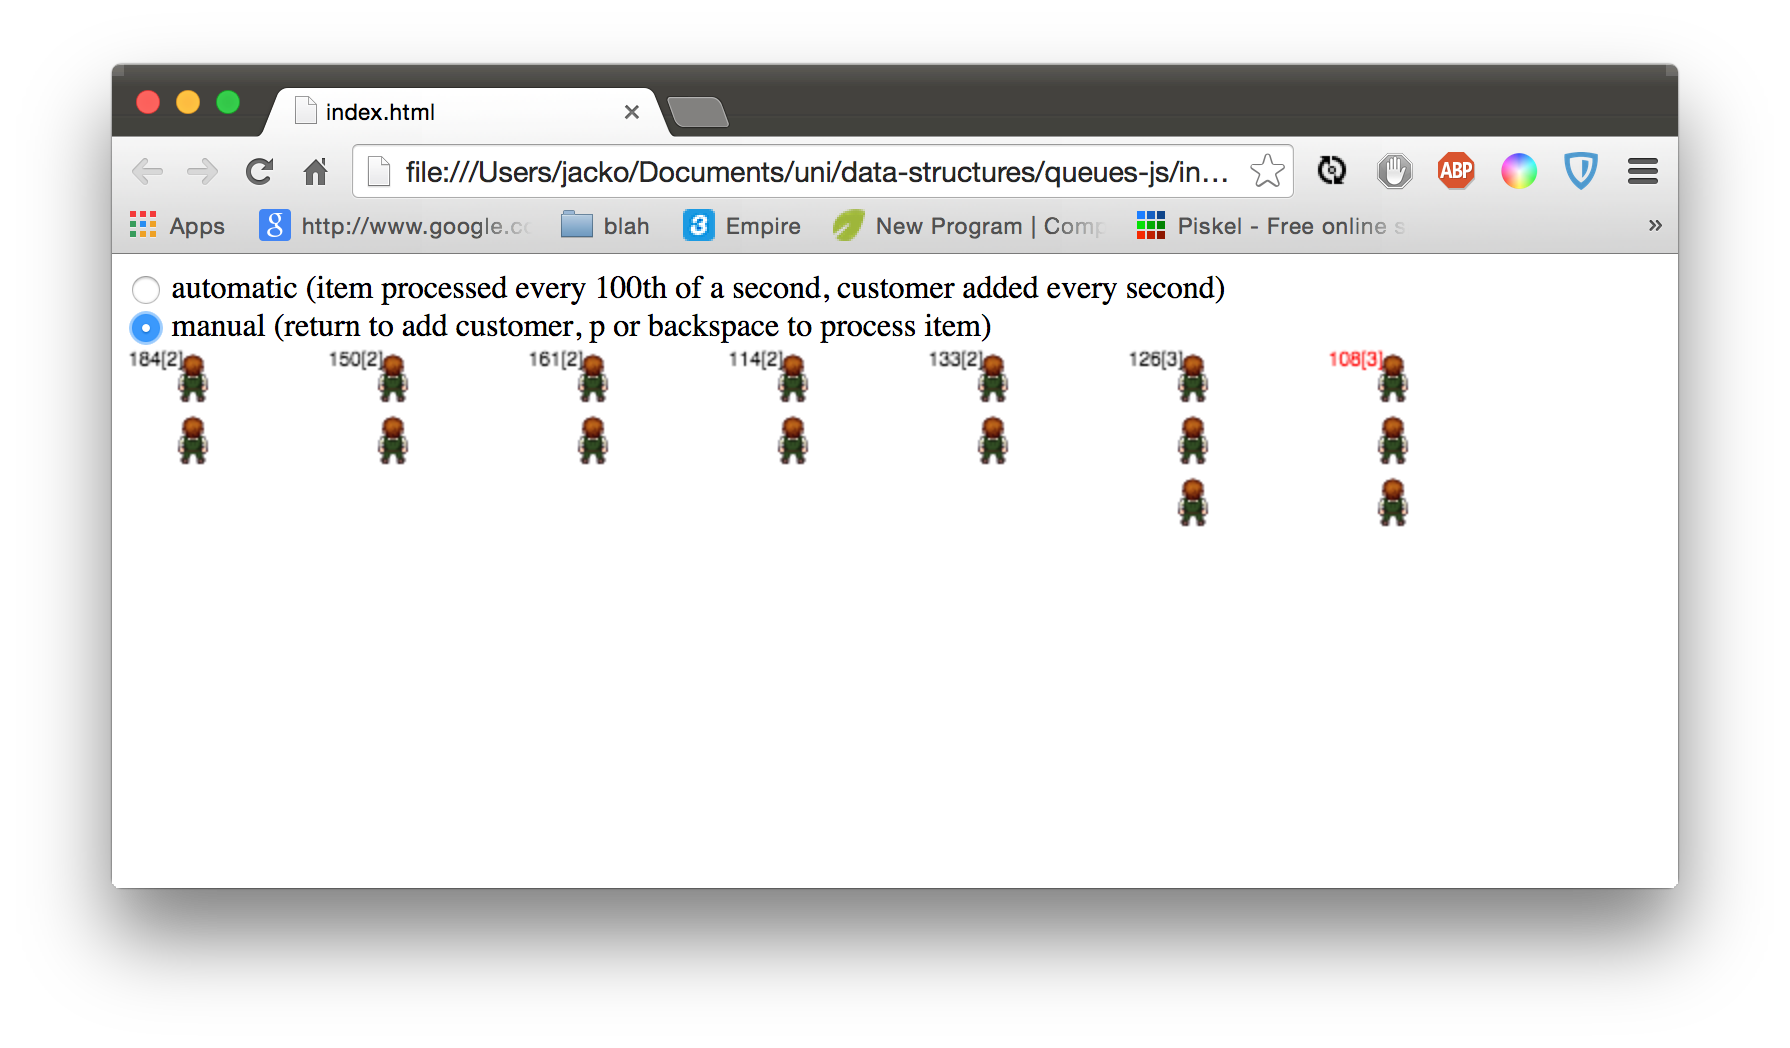
\includegraphics[width=\textwidth]{screen1.png}

After manual addition for a number of keystrokes (holding the keydown for a few seconds).

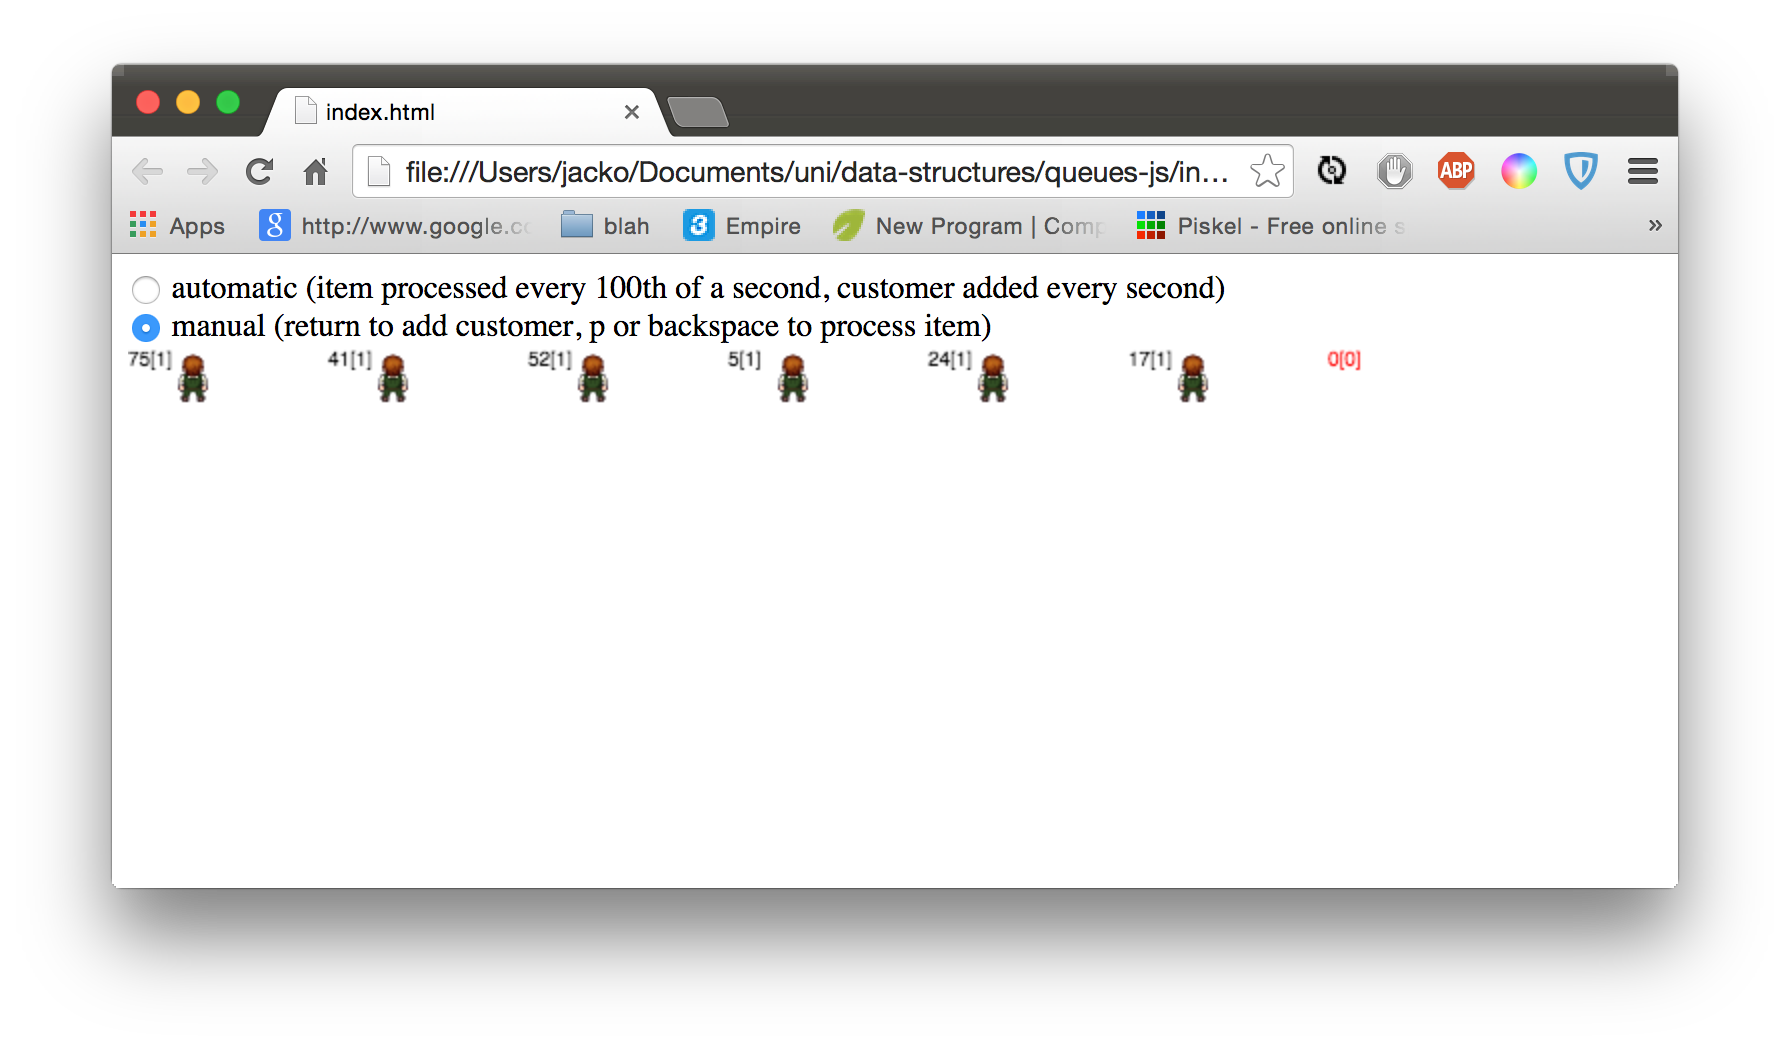
\includegraphics[width=\textwidth]{screen2.png}

Manual removal with the "p" key, aain held down for a few seconds.

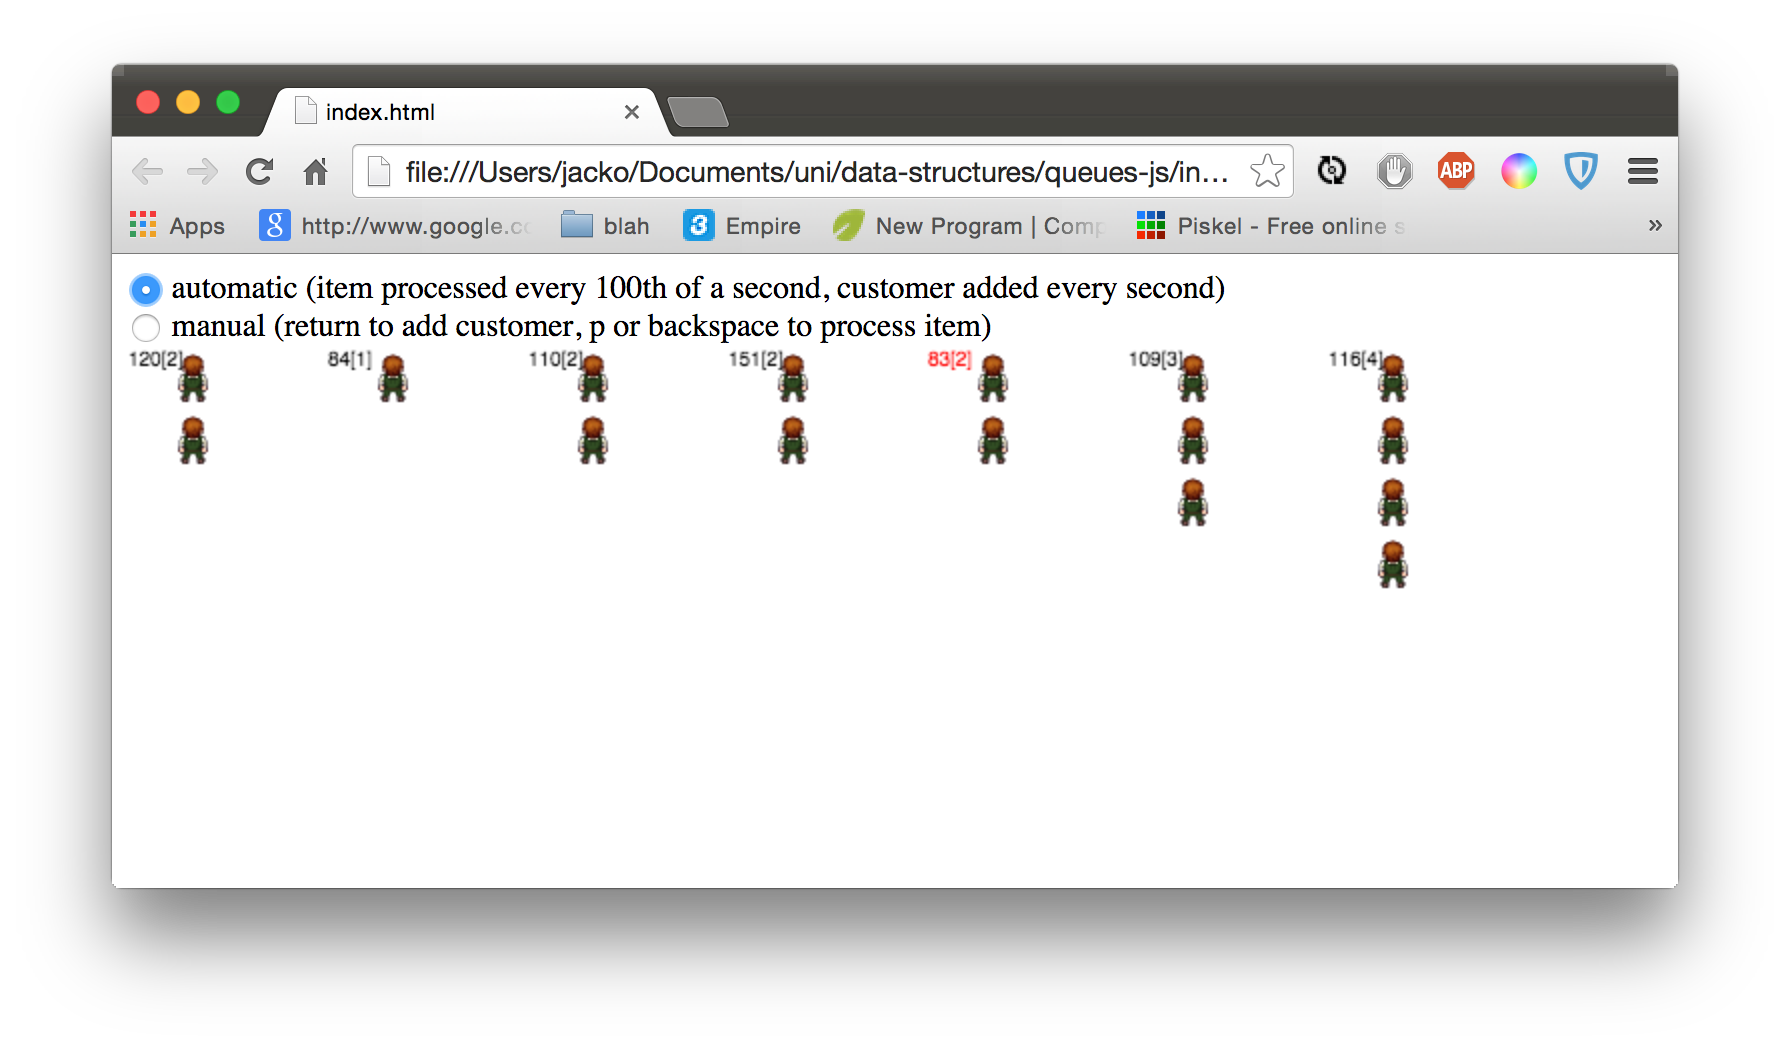
\includegraphics[width=\textwidth]{screen3.png}

Automatic processing, notice how queue 7 seems unbalanced due to people numbers, however this was down to it having the fewest items at the time the cystomer came along.

\pagebreak
\section{Evaluation}
Implementing the linked list and queue in javascript offered a rounded insight into the inner mechanics of the structures as well as being able to disregard unneeded functionality which library code may offer, such as the iterator, a queue does not need to be iterated over. 
\subsection{Single Threaded}
A major limitation of Javascript over other languages such as Java or C++ is the lack of multithreading support. Having a threadpool taking customers off queues and processing their items, while having a thread add customers would have made for a much more elegant solution. 
\subsection{Type Size (memory)}
Javascript does not stick to strict type definition, which can mean that it is more memory intensive when compared to other languages. Javascripts number type is 8 bytes which is equivalent to Java’s long primitive type. Using javas byte type would have held sufficient number values at an 8th of the memory cost.
\subsection{Other Queue Considerations} 
If more time had been possible it would have been beneficial to introduce slight variables in payment times allowing customers to further analyse the situation. Last minute changes in mind, it is possible that a customer with a small amount of items at the back of the queue may change queues after they have joind another. New lane opening, often a new checkout will open to cater to higher demand.










% End the document
\end{document}